\documentclass{article}%
\usepackage[T1]{fontenc}%
\usepackage[utf8]{inputenc}%
\usepackage{lmodern}%
\usepackage{textcomp}%
\usepackage{lastpage}%
\usepackage{authblk}%
\usepackage{graphicx}%
%
\title{Ectopic Expression of a Maize Hybrid Down{-}Regulated Gene ZmARF25 Decreases Organ Size by Affecting Cellular Proliferation in Arabidopsis}%
\author{Paula Pearson}%
\affil{Nephrology Unit, Department of Medicine, Faculty of Medicine, Thammasat University (Rangsit Campus), Khlong Nueng, Khlong Luang, Pathum Thani 12121, Thailand}%
\date{01{-}01{-}2011}%
%
\begin{document}%
\normalsize%
\maketitle%
\section{Abstract}%
\label{sec:Abstract}%
Scientists at the Swiss National Science Centre (CNS) have discovered a phenomenon called critei in ovarian cancer cells. The effect can be linked to a specific peptide molecule called bavateosphosphate. The discovery establishes the effectiveness of a countermeasure against the drug cisplatin and paclitaxel.\newline%
Critei growth affects about a quarter of patients with early{-}stage ovarian cancer and is sensitive to cisplatin. Researchers from the CSU studied ten patients who had already survived the disease. Six of the patients were resistant to cisplatin. Using an enzyme, scientists then stopped them from growing a series of tumors within a single cell. The researchers found that Critei in these patients prevented the formation of new tumors, which in turn prevented the resistance to cisplatin from spreading.\newline%
Further work will be needed to determine whether Critei growth can affect different cell types, and to identify the factors that influence its effects.\newline%
Dr. Zoltan Buzir of the State Cancer Centre of Lausanne and Prof. Walter Sylla of UCD join the author.\newline%
This research was presented in an article entitled The Effect of Critei (Critei{-}Rhodes) in the Caenorhabditis elegans and YY{-}I1{-}Brofer microglia: Countermeasure against cisplatin and paclitaxel Resistance in Ovarian Cancer Cells, recently published in the open access journal Mathematical Sciences journal.

%
\subsection{Image Analysis}%
\label{subsec:ImageAnalysis}%


\begin{figure}[h!]%
\centering%
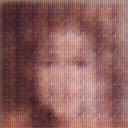
\includegraphics[width=150px]{500_fake_images/samples_5_445.png}%
\caption{A Black And White Photo Of A Black And White Cat}%
\end{figure}

%
\end{document}